%% Dokumentenklasse (Koma Script) -----------------------------------------
\documentclass[%
   11pt,              % Schriftgroesse
   ngerman,           % wird an andere Pakete weitergereicht
   a4paper,           % Seitengroesse
   DIV11,             % Textbereichsgroesse (siehe Koma Skript Dokumentation !)
]{scrartcl}%     Klassen: scrartcl, scrreprt, scrbook
% -------------------------------------------------------------------------

\usepackage[utf8]{inputenc} % Font Encoding, benoetigt fuer Umlaute
\usepackage[ngerman]{babel}   % Spracheinstellung

\usepackage[T1]{fontenc} % T1 Schrift Encoding
\usepackage{textcomp}    % Zusatzliche Symbole (Text Companion font extension)
\usepackage{lmodern}     % Latin Modern Schrift
\usepackage{listings}
\usepackage{framed}
\usepackage{amssymb}
\usepackage{amsmath}
\usepackage{framed}
\usepackage{listings}
%für die Konfusionsmatrizen
\usepackage{csvsimple}
\usepackage{lscape}


\usepackage[left=2cm,right=3cm,top=2cm,bottom=2cm,includeheadfoot]{geometry}
%Kopf- und Fußzeile
\usepackage{fancyhdr}
%Grafiken einbetten
\usepackage{graphicx}

\pagestyle{fancy}
\fancyhf{}
%Übungsteilnehmer
\fancyhead[L]{Matthias Hansen, 331600~~Lukas Huwald, 322890\\}
%Kopfzeile mittig
\fancyhead[R]{NLP Exercise03}
%Linie oben
\renewcommand{\headrulewidth}{0.5pt}

\setlength{\parskip}{1ex}

%Fußzeile links bzw. innen
\fancyfoot[L]{}
%Fußzeile rechts bzw. außen
\fancyfoot[R]{\thepage}
%Linie unten
\renewcommand{\footrulewidth}{0.5pt}
%% Dokument Beginn %%%%%%%%%%%%%%%%%%%%%%%%%%%%%%%%%%%%%%%%%%%%%%%%%%%%%%%%
\begin{document}
\section*{Task 1}
\subsection*{a.)}

See code and especially the file \texttt{README.txt}.

\subsection*{b.)}

In addition to classification accuracy, we have also plotted the percentage
of documents that the classifier rejected. Our classifier rejects a document
if p(c|document) is 0 for all classes c. In our program, this corresponds to the log-likelihood coming out as \texttt{-inf}.

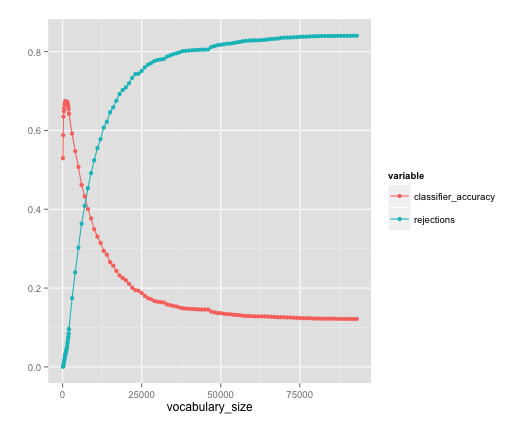
\includegraphics[width=\textwidth]{exercise03.1/accuracy_naive.png}

As we can see, the error rate shows this behavior because too many Documents are rejected due to p(c|document) being zero. This is the case because of p(document|c) being 0 in the Bayes decision rule. p(document|c) is just the product of the relative frequencies of the words of the document in the training data, however. So, to conclude, the problem is that as soon as one word that was not encountered in the training data is encountered in a test document, the test document will get rejected immediately. This occurs most frequently when the dictionary is large, because in a small dictionary, these rare words just get replaced by \texttt{<UNK>}, which is then a very frequent word.

\subsection*{c.)}

To solve this problem, we propose to use a simple smoothing method.
Originally, the class conditional probabilities of words are defined as follows:

$p(w|c) = \frac{N_{w,c}}{N_{\textunderscore,c}}$

However, the problem was that $N_{w,c}$ was zero frequently. To solve this, we simply add 1 to the occurence frequency of every word.

$p(w|c) = \frac{N_{w,c}+1}{N_{\textunderscore,c}}$

However, in this solution, the probabilites do not add up to 1, which is a problem. To fix this, we add the vocabulary size W into the normalizing factor.

$p(w|c) = \frac{N_{w,c}+1}{N_{\textunderscore,c}+W}$

We show that now this adds up to 1:

$\displaystyle\sum_w p(w|c) = \displaystyle\sum_w \frac{N_{w,c}+1}{N_{\textunderscore,c}+W} = \frac{W}{N_{\textunderscore,c}+W} + \displaystyle\sum_w \frac{N_{w,c}}{N_{\textunderscore,c}+W} = \frac{W}{N_{\textunderscore,c}+W} + \frac{N_{\textunderscore,w}}{N_{\textunderscore,c}+W} = 1$

(The penultimate step is possible because the probabilities previously added up to 1)

Now that we have solved this problem, the accuracy is much better, especially for bigger vocabularies:

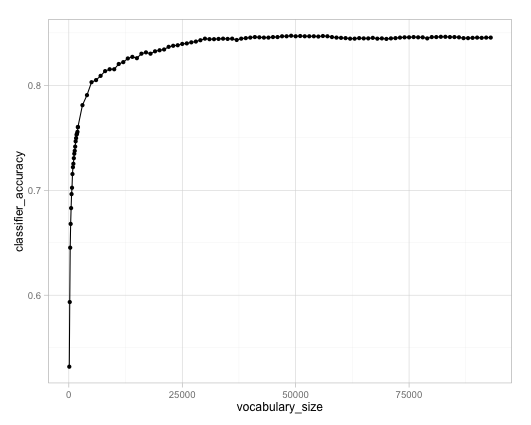
\includegraphics[width=\textwidth]{exercise03.1/accuracy_smoothed.png}


\makeatletter
\csvset{
autotabularcenter/.style={
    file=#1,
    after head=\csv@pretable\begin{tabular}{|*{\csv@columncount}{p{1.5cm}|}}\csv@tablehead,
    table head=\hline\csvlinetotablerow\\\hline,
    late after line=\\\hline,
    table foot=\\\hline,
    late after last line=\csv@tablefoot\end{tabular}\csv@posttable,
    command=\csvlinetotablerow},
}
\makeatother
\newcommand{\csvautotabularcenter}[2][]{\csvloop{autotabularcenter={#2},#1}}

\begin{landscape}
\subsection*{d.)}

Confusion matrix for smoothed probabilities:

\scalebox{0.5} {
    \csvautotabularcenter{exercise03.1/confusion_matrix_smoothed.csv}
}
\end{landscape}

\begin{landscape}

Confusion matrix for unsmoothed probabilities:

\scalebox{0.5} {
    \csvautotabularcenter{exercise03.1/confusion_matrix.csv}
}
\end{landscape}

As we can see, in the unsmoothed case most documents just get rejected.

In the smoothed case, most documents are classified correctly, as shown by the high numbers in the diagonal. The cases where the classifier indeed makes mistakes are newsgroups, that are very similar, like \texttt{talk.politics.misc} and \texttt{talk.politics.guns}.


\subsection*{e.)}

See Code. The classifier achieves a classification accuracy of roughly 90\%

\section*{Task 2}
For $N = 0$, we get that
\begin{equation*}
	p(0) = \sum_{w_1^0}p(w_1^0\$) = p(\$)
\end{equation*}
with the assumption that there is a unique string of length 0 ($\varepsilon$).\par
For $N > 1$ we get
\begin{align*}
	p(N) = \sum_{w_1^N} p(w_1^N\$) &= \sum_{w_1^N} \bigg(\prod_{i=1}^N p(w_i|h_i)\bigg) \cdot p(\$) \\
	&= p(\$) \cdot \sum_w \sum_{w_1^N\colon w_N = w} \bigg(\prod_{i=1}^{N-1} p(w_i|h_i)\bigg) \cdot p(w|h_N) \\
	&= p(\$) \cdot \sum_w \sum_{w_1^{N-1}} \bigg(\prod_{i=1}^{N-1} p(w_i|h_i)\bigg) \cdot p(w|h_N) \\
	&= p(\$) \cdot \sum_{w_1^{N-1}} \sum_w \bigg(\prod_{i=1}^{N-1} p(w_i|h_i)\bigg) \cdot p(w|h_N) \\
	&= p(\$) \cdot \sum_{w_1^{N-1}} \bigg(\prod_{i=1}^{N-1} p(w_i|h_i)\bigg) \cdot (\sum_w p(w|h_N)) \\
	&= \sum_{w_1^{N-1}} \bigg(\prod_{i=1}^{N-1} p(w_i|h_i)\bigg) \cdot p(\$) \cdot (1 - p(\$)) \\
	&= p(N-1) \cdot (1 - p(\$))
\end{align*}
and thus
\begin{equation*}
	p(N) = (1 - p(\$))^N \cdot p(\$)
\end{equation*}
This distribution is normalized as
\begin{equation*}
	\sum_N p(N) = \sum_N (1 - p(\$))^N \cdot p(\$) = p(\$) \cdot \sum_N (1 - p(\$))^N = p(\$) \cdot \frac{1}{1 - (1 - p(\$))} =1
\end{equation*}
\section*{Task 3}
From the slides we have the log likelihood function
\begin{equation*}
	F(\{\lambda_h\}) = \sum_h \bigg[N_1(h,\cdot)\cdot\text{log}(\lambda_h) + (N(h,\cdot) - N_1(h, \cdot))\cdot \text{log}(1 - \lambda_h)\bigg]
\end{equation*}
We can do independent optimization for each $h$ as there is no dependence between parameters. So for a single $\lambda_h$ we need to maximize
\begin{equation*}
	\hat{F}(\lambda_h) = N_1(h,\cdot)\cdot\text{log}(\lambda_h) + (N(h,\cdot) - N_1(h, \cdot))\cdot \text{log}(1 - \lambda_h)
\end{equation*}
which after multiplying with the constant $\frac{1}{N(h,\cdot)}$is equivalent to maximizing
\begin{equation*}
	\tilde{F}(\lambda_h) = \frac{N_1(h,\cdot)}{N(h,\cdot)}\cdot\text{log}(\lambda_h) + (1 - \frac{N_1(h,\cdot)}{N(h,\cdot)})\cdot \text{log}(1 - \lambda_h)
\end{equation*}
Now $\frac{N_1(h,\cdot)}{N(h,\cdot)}$ and $1 - \frac{N_1(h,\cdot)}{N(h,\cdot)}$ form a probability distribution $p_k$, and using the divergence inequality
\begin{equation*}
	\sum_k p_k \cdot\text{log}(q_k) \leq \sum_k p_k \cdot\text{log} (p_k)
\end{equation*}
with $q_k = \{\lambda_h, 1 - \lambda_h\}$ we see that the optimal estimate is 
\begin{equation*}
	\lambda_h = \frac{N_1(h,\cdot)}{N(h,\cdot)}
\end{equation*}
\section*{Task 4}
Again we start with the log likelihood function
\begin{align*}
	F(\{\lambda_h\}) &= \sum_h \bigg[N_1(h,\cdot)\cdot\text{log}(\lambda_h) + (N(h,\cdot) - N_1(h, \cdot))\cdot \text{log}(1 - \lambda_h)\bigg] \\
	&= \sum_N \sum_{h\colon N(h,\cdot) = N} \bigg[N_1(h,\cdot)\cdot\text{log}(\lambda_N) + (N(h,\cdot) - N_1(h, \cdot))\cdot \text{log}(1 - \lambda_N)\bigg] 
\end{align*}
We can do independent optimization for each $N$ as there is no dependence between parameters for different counts. So for a single $N$ we need to maximize
\begin{equation*}
	\hat{F}(\lambda_N) = \sum_{h\colon N(h,\cdot) = N} \bigg[N_1(h,\cdot)\cdot\text{log}(\lambda_N) + (N(h,\cdot) - N_1(h, \cdot))\cdot \text{log}(1 - \lambda_N)\bigg] 
\end{equation*}
which after multiplying with the constant $\frac{1}{\sum_{h\colon N(h,\cdot) = N}N(h,\cdot)}$is equivalent to maximizing
\begin{equation*}
	\tilde{F}(\lambda_N) = \frac{\sum_{h\colon N(h,\cdot) = N}N_1(h,\cdot)}{\sum_{h\colon N(h,\cdot) = N}N(h,\cdot)}\cdot\text{log}(\lambda_N) + (1 - \frac{\sum_{h\colon N(h,\cdot) = N}N_1(h,\cdot)}{\sum_{h\colon N(h,\cdot) = N}N(h,\cdot)})\cdot \text{log}(1 - \lambda_N)
\end{equation*}
We again use divergence inequality like in task 3 and find that the optimal estimate is
\begin{equation*}
	\lambda_N = \lambda_{N(h,\cdot)} = \frac{\sum_{h\colon N(h,\cdot) = N}N_1(h,\cdot)}{\sum_{h\colon N(h,\cdot) = N}N(h,\cdot)}
\end{equation*}
\end{document}
